\documentclass[10pt]{article}
\usepackage[english]{babel}
\usepackage{amsmath}
\usepackage{graphicx}
\usepackage[colorinlistoftodos]{todonotes}
\pagestyle{headings}
\usepackage{indentfirst}
\usepackage[utf8]{inputenc}
\usepackage{xeCJK}
\usepackage{float}

%% Code blocl setting
\usepackage{listings}
\renewcommand{\lstlistingname}{Code}% Listing -> Algorithm
\usepackage{color}

\definecolor{dkgreen}{rgb}{0,0.6,0}
\definecolor{gray}{rgb}{0.5,0.5,0.5}
\definecolor{mauve}{rgb}{0.58,0,0.82}

\lstset{frame=tb,
  language=Python,
  aboveskip=3mm,
  belowskip=3mm,
  showstringspaces=false,
  columns=flexible,
  basicstyle={\small\ttfamily},
  numbers=none,
  numberstyle=\tiny\color{gray},
  keywordstyle=\color{blue},
  commentstyle=\color{dkgreen},
  stringstyle=\color{mauve},
  breaklines=true,
  breakatwhitespace=true,
  tabsize=3
}

\begin{document}

\begin{titlepage}

\newcommand{\HRule}{\rule{\linewidth}{0.5mm}} % Defines a new command for the horizontal lines, change thickness here

\center % Center everything on the page

%----------------------------------------------------------------------------------------
%	HEADING SECTIONS
%----------------------------------------------------------------------------------------

\textsc{\LARGE Shanghai Jiaotong University}\\[1.5cm] % Name of your university/college
\textsc{\Large Big Data Processing Technology}\\[0.5cm] % Major heading such as course name
%\textsc{\large Minor Heading}\\[0.5cm] % Minor heading such as course title

%----------------------------------------------------------------------------------------
%	TITLE SECTION
%----------------------------------------------------------------------------------------

\HRule \\[0.4cm]
{ \huge \bfseries Project 3: Mini DFS}\\[0.4cm] % Title of your document
\HRule \\[1.5cm]

%----------------------------------------------------------------------------------------
%	AUTHOR SECTION
%----------------------------------------------------------------------------------------

\begin{minipage}{0.4\textwidth}
\begin{flushleft} \large
\emph{Author:}\\
% Your name
FEI Yixiao \\118260910031\\
LI Yanhao \\118260910036\\
LUO Dihao \\118260910039\\ % Your name
SHEN Shengyang \\118260910042\\
YAN Shuhan \\118260910050\\ % Your name
\end{flushleft}
\end{minipage}
~
\begin{minipage}{0.4\textwidth}
\begin{flushright} \large
\emph{Supervisor:} \\
Chentao  \textsc{WU} \\% Supervisor's Name
Xin  \textsc{XIE}
\end{flushright}
\end{minipage}\\[2cm]

% If you don't want a supervisor, uncomment the two lines below and remove the section above
%\Large \emph{Author:}\\
%John \textsc{Smith}\\[3cm] % Your name

%----------------------------------------------------------------------------------------
%	DATE SECTION
%----------------------------------------------------------------------------------------

{\large \today}\\[2cm] % Date, change the \today to a set date if you want to be precise

%----------------------------------------------------------------------------------------
%	LOGO SECTION
%----------------------------------------------------------------------------------------


\includegraphics[width=0.5\textwidth]{logo_SPEIT.jpg}\\[1cm] % Include a department/university logo - this will require the graphicx package

%----------------------------------------------------------------------------------------

\vfill % Fill the rest of the page with whitespace

\end{titlepage}
\indent

\section{Introduction}

Our distributed metadata management is based on Java and is composed with following files:

\begin{itemize}
  \item Client
  \begin{itemize}
    \item Client.java : the client interface where commands are accepted
  \end{itemize}
  \item Cluster
  \begin{itemize}
    \item Cluster.java : we use this class to group data servers and distribute data blocks
    \item DataServer.java : distributed data servers which stores  eventually data blocks
    \item MetaData.java : store meta data information
    \item DirectoryTree.java : directory tree information
    \item TreeNode.java : tree node information
  \end{itemize}
  \item Tools
  \begin{itemize}
    \item Request.java : class to define the message
    \item Response.java : class to define the message
  \end{itemize}
\end{itemize}

\subsection{Usage}

Users can access distributed metadata management by directly running \textit{Client.class}. Before that, we need 
to also launch the management services including the \textit{Cluster.class} and at least one \textit{DataServer.class}.

\begin{itemize}
  \item cd dir\_name : go to the directory
  \item ls : show list of files and directories
  \item touch file\_name : create a file with with the name of file\_name
  \item mkdir dir\_name : create a directory with the name of dir\_name
  \item tree : show the tree structure of the files and directories
  \item fulltree : show the tree structure of the files and directories with full paths
  \item chkdist : check distributed metadata in all data servers
  \item stat file\_name : check the permissions of a file
  \item chmod file\_name permissions: modify the permissions of a file
  \item exit : exit distributed metadata management
\end{itemize}

When a client sends a command to the interface \textit{Client}, 
\textit{Client} shares this command with \textit{Cluster} and \textit{DataServer} through \textit{Request} and \textit{Response}. 
\textit{Cluster} will choose either an appropriate \textit{DataServer} to store the data block or extract the information it 
needs and gives back the information to the \textit{Client}.
\section{Example}

As you may discover during the experiment, our distributed metadata management accepts only several commands. 
When the command line does not understand the command, it gives the list of the accepted commands. 
In addition, each command has its own format of the input. The input number of arguments might be different, 
so when the format is not correct, it also gives the warning message to help the client enter the correct commands.\\ 
Now first, we can create several files in our distributed metadata management using \textit{touch} 
and then we can also create some directories using \textit{mkdir}.

\begin{figure}[H]
\centerline{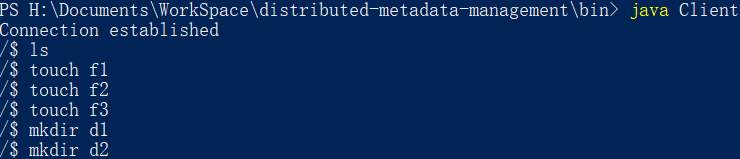
\includegraphics[width = 1\textwidth]{images//1 create.png}}
\caption{Usage: touch \& mkdir}
% \label{fig_process}
\end{figure}

In directory \textit{bin/test1} and also in \textit{bin/test2}, we can see that it creates some blocks. 
These two directories are generated by the \textit{DataServer} whose names are respectively \textit{test1} and \textit{test2}.

\begin{figure}[H]
\centerline{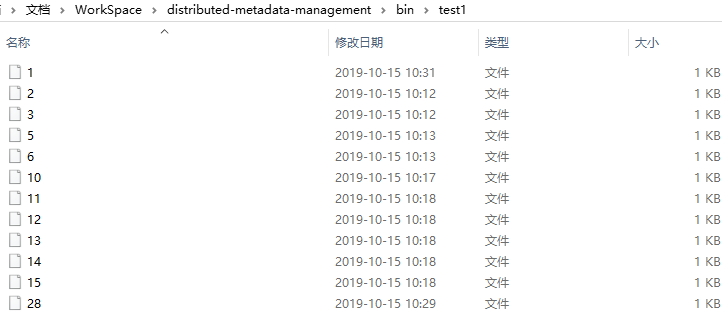
\includegraphics[width = 1\textwidth]{images//10 files.png}}
\caption{Usage: put \& mkdir}
% \label{fig_process}
\end{figure}

Then, we can try to list what we have created for now. As you can see in the presented picture, we have created three files and 
three directories with the timestamp respectively.

\begin{figure}[H]
\centerline{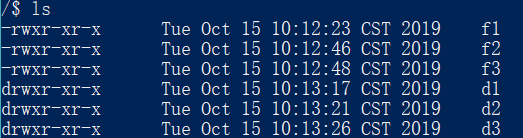
\includegraphics[width = 1\textwidth]{images//2 list.png}}
\caption{Usage: ls}
% \label{fig_process}
\end{figure}

Now let us create more files and directories to complicate our metadata management and 
we will use \textit{tree} to display the structure.

\begin{figure}[H]
\centerline{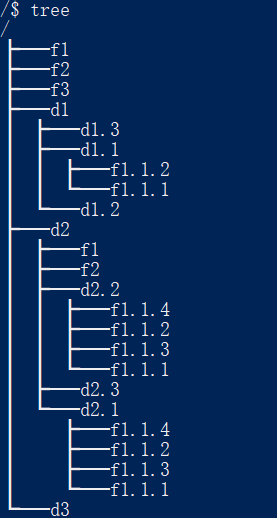
\includegraphics[width = 0.5\textwidth]{images//4 tree.png}}
\caption{Usage: tree}
% \label{fig_process}
\end{figure}

And \textit{fulltree} will display the structure with the complete paths.

\begin{figure}[H]
\centerline{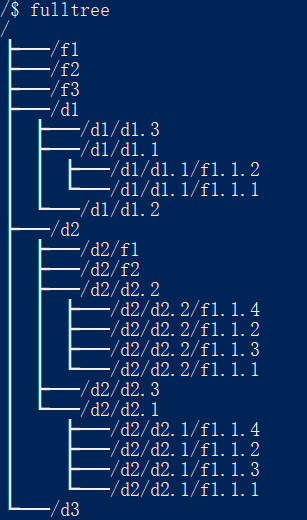
\includegraphics[width = 0.5\textwidth]{images//3 fulltree.png}}
\caption{Usage: fulltree}
% \label{fig_process}
\end{figure}

Since we have a relatively complicated file structure, now we can check where these 
data nodes are stored in our distributed metadata management using \textit{chkdist}.

\begin{figure}[H]
\centerline{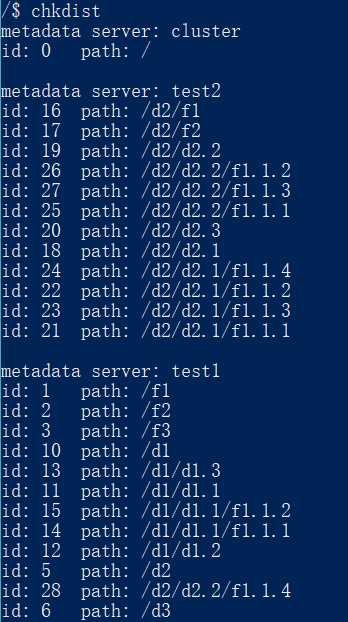
\includegraphics[width = 0.5\textwidth]{images//5 chkdist.png}}
\caption{Usage: chkdist}
% \label{fig_process}
\end{figure}

We can of course change the permissions and check whether our modification works. To do this, 
we first check the permissions with \textit{stat}. Then we change the permissions with \textit{chmod}. 
and finally, we check once again the permissions.

\begin{figure}[H]
\centerline{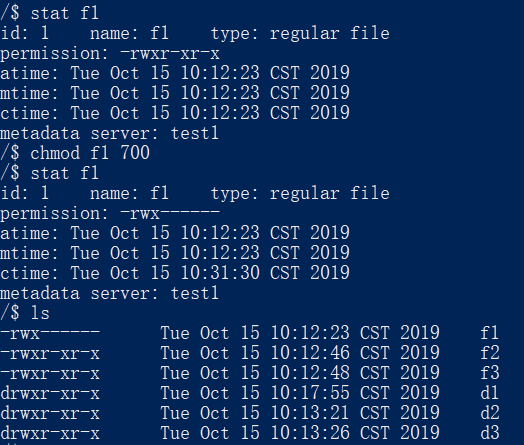
\includegraphics[width = 0.7\textwidth]{images//6 stat and chmod.png}}
\caption{Usage: stat \& chmod}
% \label{fig_process}
\end{figure}

Now we wonder what if one of our \textit{DataServer} goes offline. Here we did an experiment by disabling \textit{DataServer test2}. 
And we knew in advance that all the data blocks related to files in \textit{d2} are stored exactly in \textit{DataServer test2}. 
Naturally, we will go into \textit{d2} to see what would happen. As you might observe in the picture, this time when we demand 
listing the files in \textit{d2}, it could not extract information though the tree information is still stored in the \textit{TreeNode}.

\begin{figure}[H]
\centerline{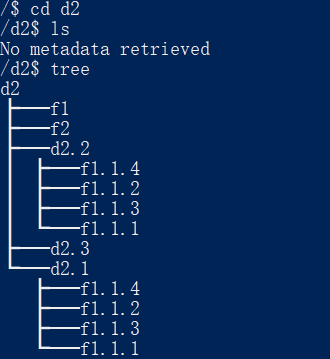
\includegraphics[width = 0.5\textwidth]{images//7 when test2 is offline.png}}
\caption{When test2 is offline}
% \label{fig_process}
\end{figure}

Now we can make \textit{DataServer test2} go online once again. This time when we demand 
listing the files in \textit{d2}, it could extract information, which is exactly what we want.

\begin{figure}[H]
\centerline{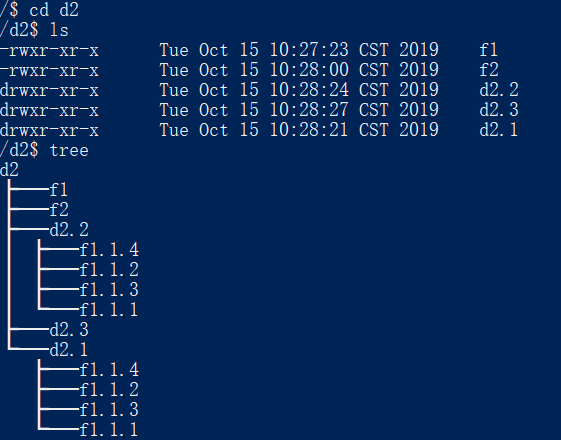
\includegraphics[width = 0.7\textwidth]{images//8 when test2 is realive.png}}
\caption{When test2 is re-alive}
  % \label{fig_process}
\end{figure}

Finally, we can safely exit distributed metadata management and this completes our examples of the experiment.

\begin{figure}[H]
\centerline{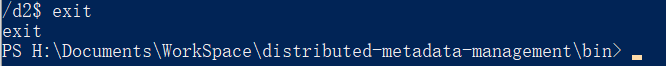
\includegraphics[width = 1\textwidth]{images//9 exit.png}}
\caption{Usage: quit}
% \label{fig_process}
\end{figure}

% \begin{figure}[h]
% \centerline{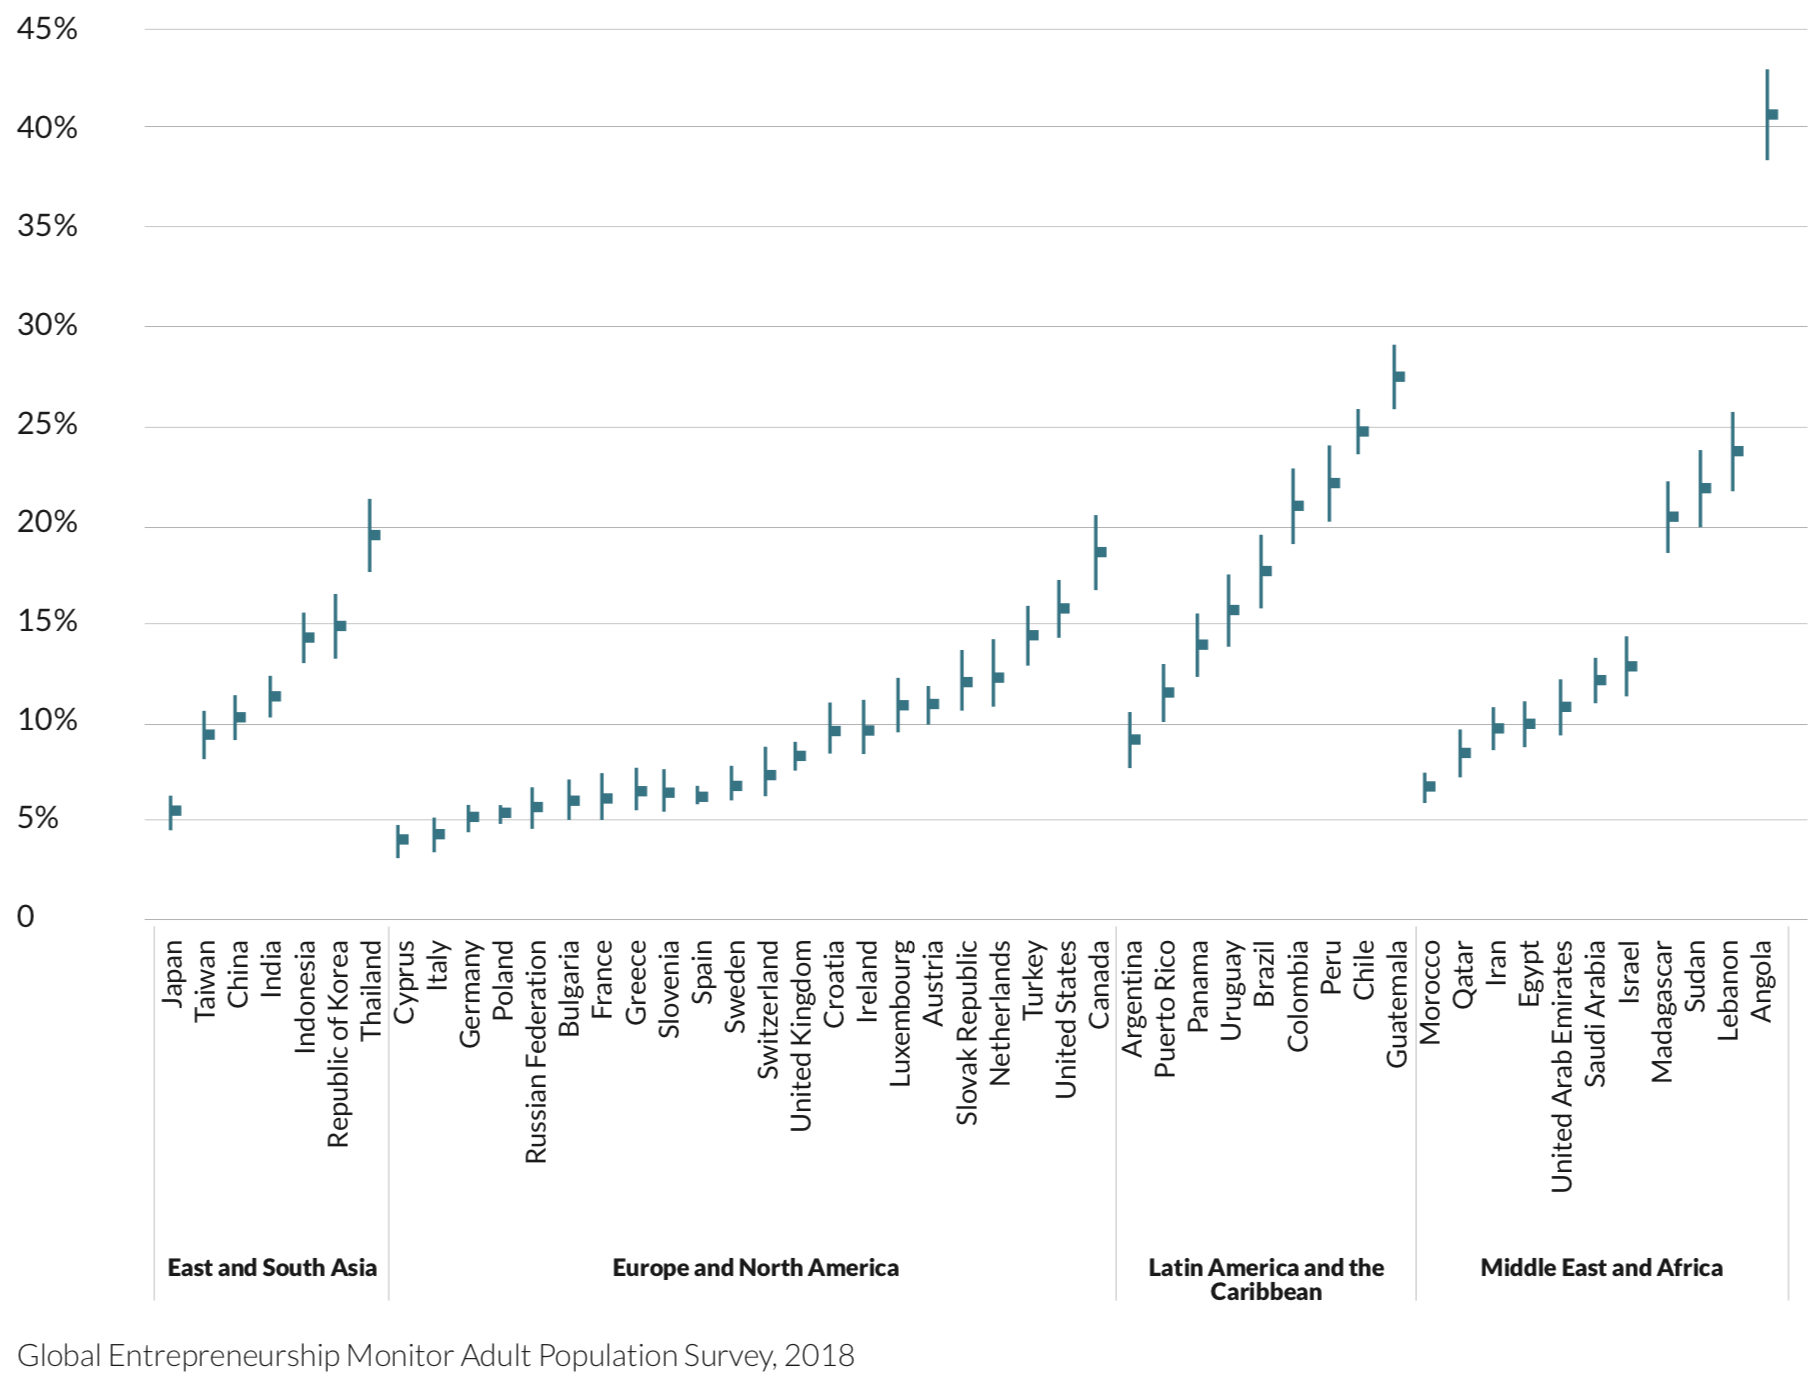
\includegraphics[width = 1\textwidth]{screenshot//2_2.png}}
% \caption{Total early-stage Entrepreneurial Activity (TEA) Rates among Adults (ages 18-64) in 487 Economies, in Four Geographic Regions}
% \label{fig_TEA_global}
% \end{figure}

% \section{Pod}
% \subsection{1 Pod with 1 Container}
%
% We can see after creating pod1 by pod1.yaml, we can execute any command by kubectl exec -it pod1 -- command.
%
% \begin{figure}[H]
% \centerline{\includegraphics[width = 0.7\textwidth]{screenshot//1.png}}
% \caption{1 Pod with 1 Container}
% % \label{fig_1pod1container}
% \end{figure}
%
% \subsection{1 Pod with 2 Containers}
%
% We can see after we change index.html in container ct-debian, we can also see the change in container ct-nginx.
%
% \begin{figure}[H]
% \centerline{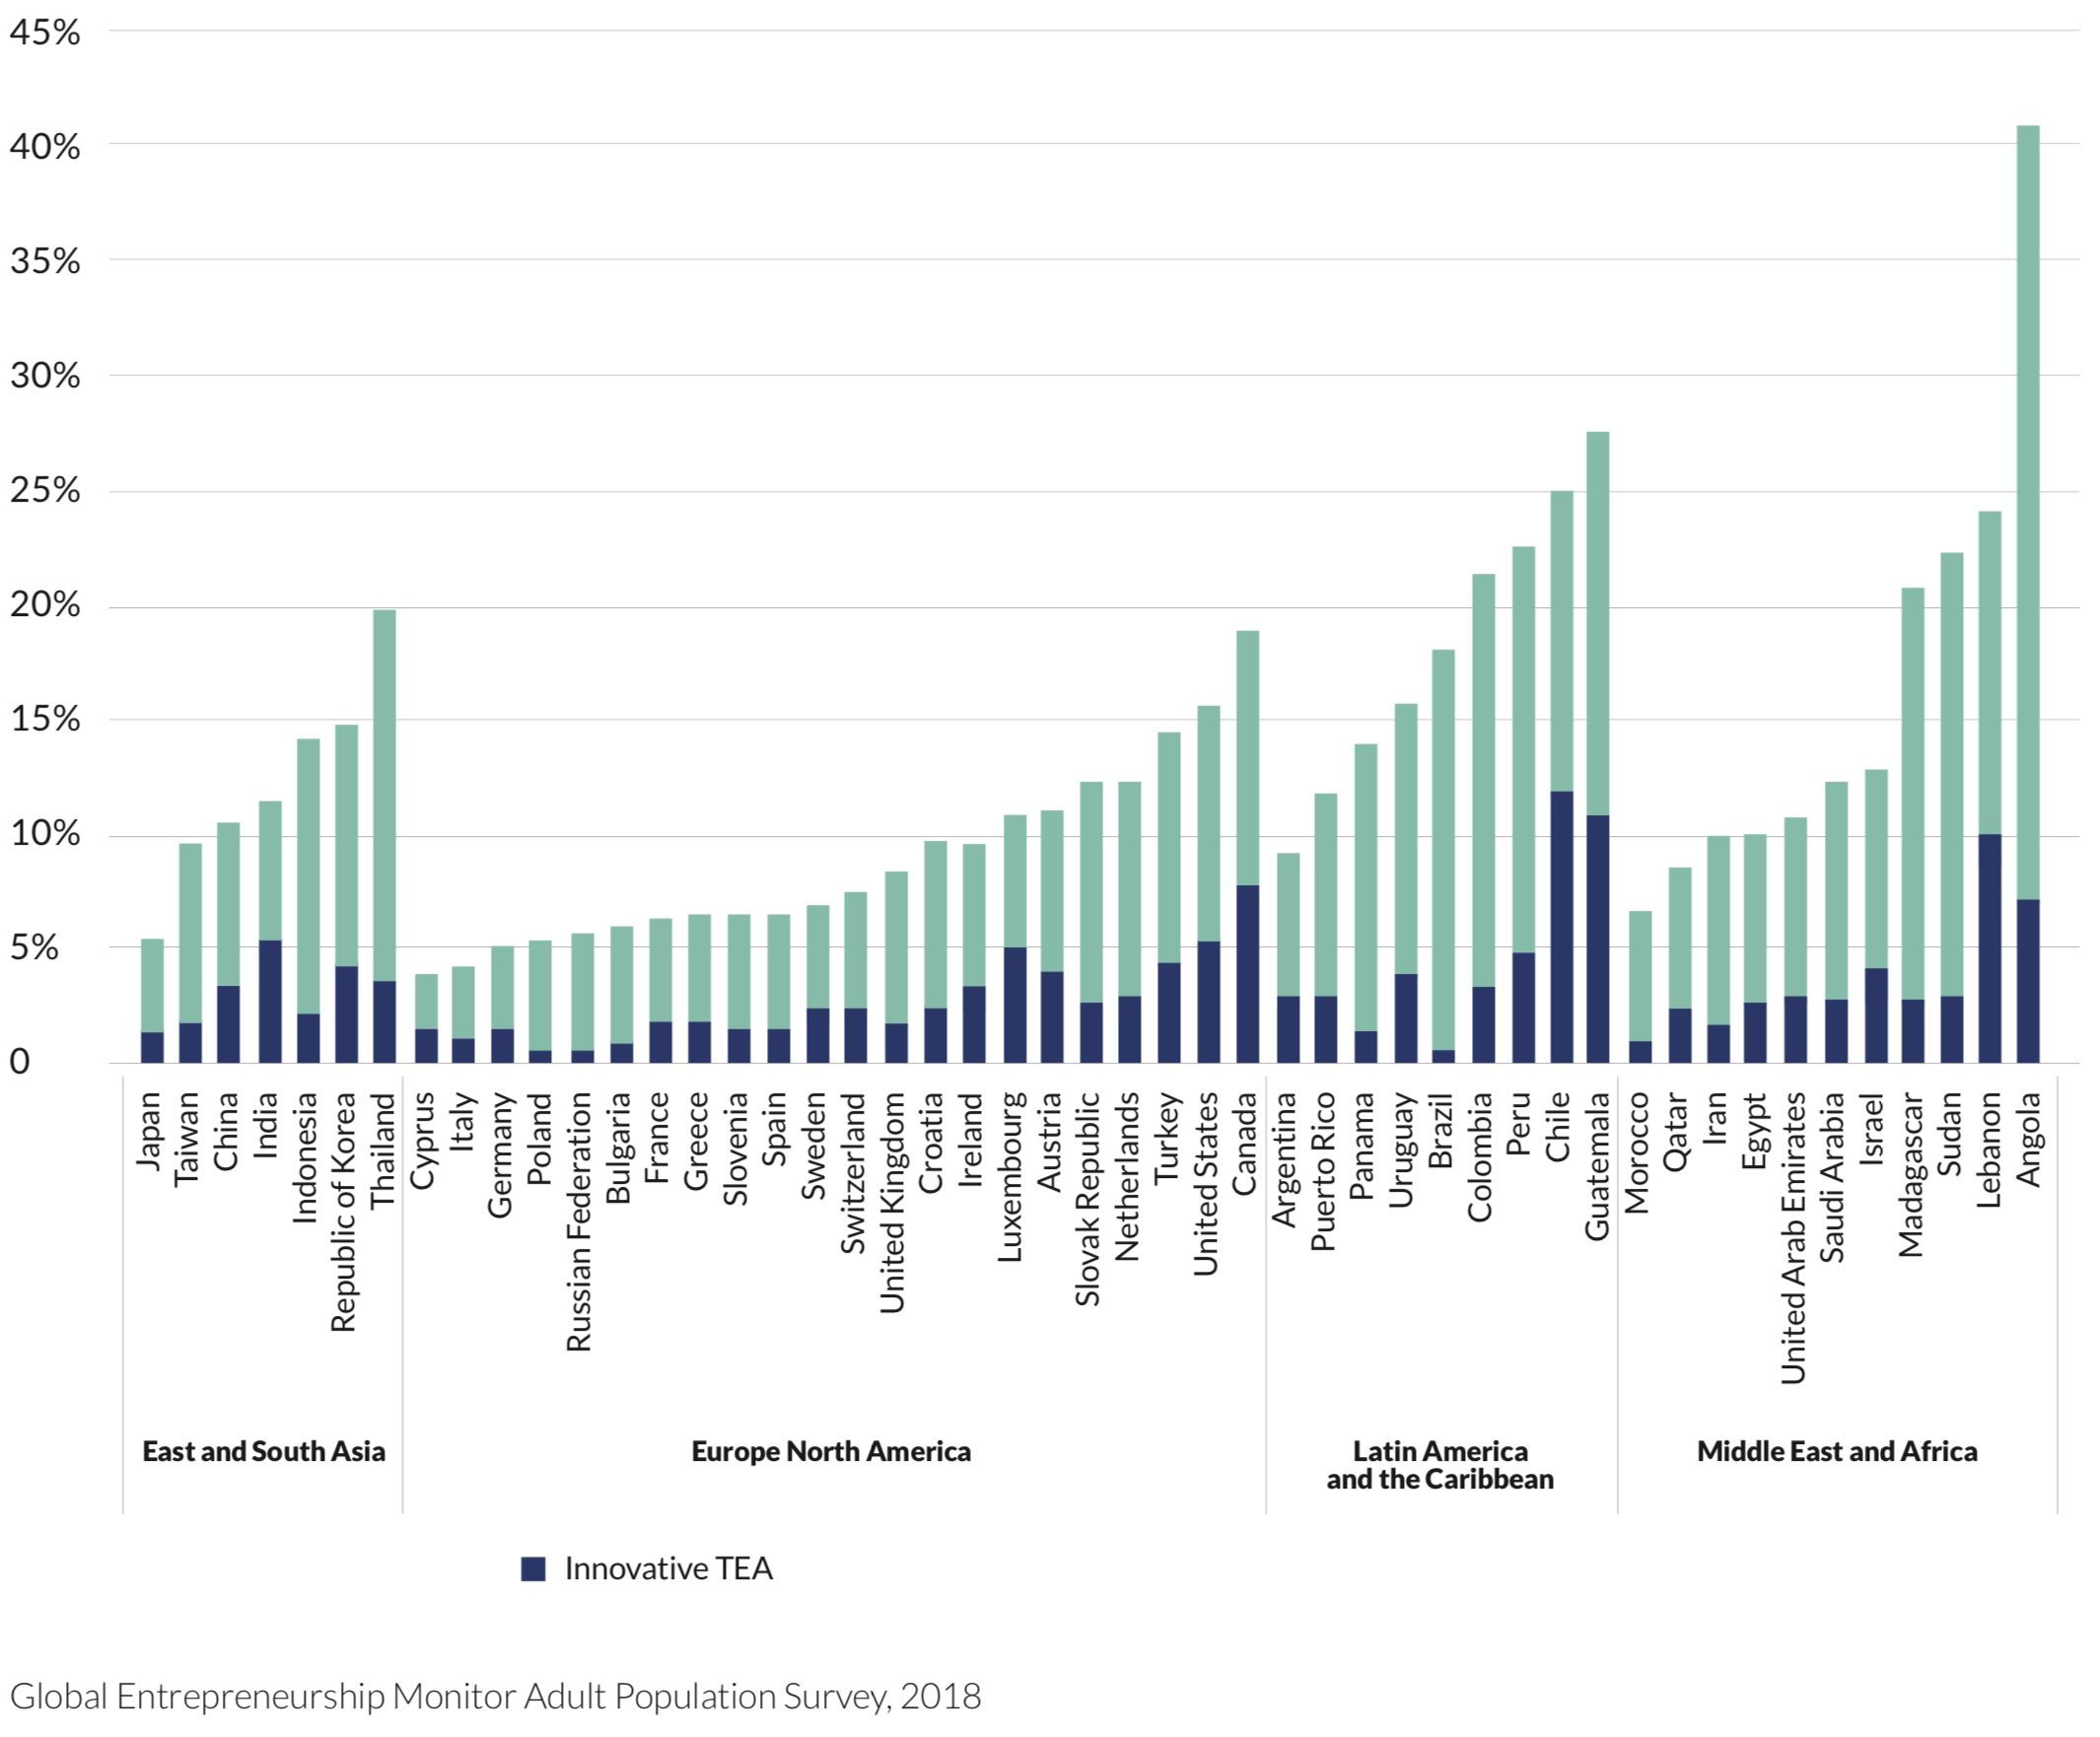
\includegraphics[width = 0.7\textwidth]{screenshot//2_1.png}}
% \caption{1 Pod with 2 Container}
% % \label{fig_1pod1container}
% \end{figure}






\end{document}
